\documentclass{article}
\usepackage[final]{nips_2018}
\usepackage[utf8]{inputenc}
\usepackage[T1]{fontenc}

\usepackage{hyperref}
\usepackage{url}
\usepackage{bm}
\usepackage{booktabs}
\usepackage{amsfonts}
\usepackage{nicefrac}
\usepackage{enumerate}
\usepackage{microtype}
\usepackage{graphicx}
\usepackage{subfigure}
\usepackage{amsmath}
\usepackage{amsthm}
\usepackage{caption}
\usepackage{multirow}
\usepackage{enumitem}
\usepackage{listings}
\usepackage{todonotes}
\usepackage{mathtools}

\renewcommand{\thesubsubsection}{\thesubsection\,\alph{subsubsection})}
\newcommand{\del}[2]{\ensuremath{\frac{\partial #1}{\partial #2}}}
\newcommand{\Ell}{\ensuremath{\mathcal{L}}}

% for absolute value notation
\DeclarePairedDelimiter\abs{\lvert}{\rvert}
\makeatletter
\let\oldabs\abs
\def\abs{\@ifstar{\oldabs}{\oldabs*}}
\let\oldnorm\norm
\def\norm{\@ifstar{\oldnorm}{\oldnorm*}}
\makeatother

\lstset{basicstyle=\ttfamily\footnotesize,breaklines=true}

\title{\textbf{Assignment 3}\\Deep Generative Models}

\author{
  Francesco Dal Canton \\
  \texttt{f.dal.canton@student.uva.nl} \\
  12404225
}

\begin{document}

\maketitle

%################################# NEW SECTION ##################################
\section{Variational Auto Encoders}

%###################### NEW SUBSECTION #######################
\subsection{Latent Variable Models}

\begin{enumerate}[label=\textbf{1.\arabic*}]
  \item

  \begin{enumerate}[label=\arabic*.]
    \item
    VAEs and VAs are different in terms of their main function.

    VAs are used for dimensionality compression: the encoder and the decoder are part of a single network which approximates the identity function. Since the network as a bottleneck between encoder and decoder, the activations of that bottleneck serve as reduced features for the input. While the decoder part of the network may be used for generation, by providing some random features for the bottleneck layer, we can't sample from the distribution of the data.

    A VAE works differently, since it is a generative model. VAEs still use a bottleneck structure, but in this case the encoder learns the data's probability distribution, which makes it possible to sample from said distribution and generate an output similar to the input sample. In that sense, the decoder of a VAE works similarly as to that of a VA.

    \item
    This was answered in the previous question. Since VAs don't model the data's distribution (be it mapped to a latent space or not), they are not generative models.

    \item
    One of the main purposes of AEs is to produce a reduced dimensionality version of the input sample. This means that the encoder should be able to map each sample to a tensor of reduced dimensionality. Since VAEs model a distrubution over the data instead of specific latent representations for single samples, it might be possible to use them for data compression if we take the distribution parameters to be the features of the compressed input.

    \item
    This was answered in the first question. VAEs are generative since they explicitly model the distribution of the data (or, rather, the distribution of the latent variables), while VAs don't.

  \end{enumerate}
\end{enumerate}

%###################### NEW SUBSECTION #######################
\subsection{Decoder: The Generative Part of the VAE}

\begin{enumerate}[label=\textbf{1.\arabic*}]
  \setcounter{enumi}{1}
  \item
  The procedure used to sample from such a model is, as mentioned, ancestral sampling. This technique may be applied to any graphical model expressing variable dependencies. The idea is that we first sample from variables that do not depend on others, and once we have sampled those, we may sample the ones that depend on them. This can be repeated iteratively until we have sampled all variables in the model.

  In our case we only have two variables $\bm{z}_n$ and $\bm{x}_n$, where the latter depends on the former. This means that we first sample $\bm{z}_n \sim \mathcal{N}(0, \bm{I}_D)$, which allows us to use the sampled $\bm{z}_n$ in order to sample $p(\bm{x}_n | \bm{z}_n)$ according to equation:

  \begin{align*}
    p(\bm{x}_n | \bm{z}_n) &= \prod_{m=1}^M \text{Bern} \left( \bm{x}_n^{(m)} | f_{\theta} (\bm{z}_n)_m \right)
  \end{align*}

  \item
  The key element that makes it so that the assumption is not restrictive is the term $f_{\theta} (\bm{z}_n)_m$ in the equation above. This term indicates that, when computing $p(\bm{x}_n | \bm{z}_n)$, we are actually using a parametric function of $\bm{z}_n$ as its input. Carl Doersch's tutorial reminds us that if this function is complex enough, we can map a normally distributed $p(\bm{z}_n)$ to any $n$-dimensional distribution. We can assume that the VAE's decoder's first few layers will perform exactly this operation, mapping the latent variables to the actual distribution of the data before it is reconstructed.

  \item

  \begin{enumerate}[label=(\alph*)]
    \item
    We can approximate $\log p(\bm{x}_n)$ using Monte-Carlo Integration as follows:

    \begin{align*}
      \log p(\mathcal{D}) &= \sum_{n=1}^{N} \log \int \log p(\bm{x}_n | \bm{z}_n) p(\bm{z}_n) d \bm{z}_n \\
      &\approx \sum_{n=1}^{N} \log \frac{1}{N} \sum_{i=1}^{S} p\left[\bm{x}_n | \bm{z}_n^{(i)}\right] \quad \text{with} \quad \bm{z}_n^{(i)} \sim p(\bm{z}_n) \\
      &\approx \sum_{n=1}^{N} \log \frac{1}{N} \sum_{i=1}^{S} \prod_{m=1}^M \text{Bern} \left( \bm{x}_n^{(m)} | f_{\theta} \left[ \bm{z}_n^{(i)} \right]_m \right)
    \end{align*}

    Where $S$ is the total number of samples we will take when computing the approximation.

    \item
    The inefficiency problem that this method brings boils down to the issue of sparsity in high-dimensional spaces. In order to approximate $\log p(\bm{x}_n)$, we sample a number of $\bm{z}_n^{(i)} \sim p(\bm{z}_n)$. As the dimensionality of $\bm{z}$ increases, however, the search space increases exponentially. This in turn means that we need many more samples to properly approximate $\log p(\bm{x}_n)$, making the procedure inefficient.

    This problem is made worse by the presence of the $p(\bm{x}_n | \bm{z}_n)$ in the integral above. Even if we sample $\bm{z}_n^{(i)}$, it might be that $p(\bm{x}_n | \bm{z}_n)$ is incredibly small given the sparsity of the high-dimensional space. This means that the calculation will have almost no impact on the learning procedure, and it will have the only effect of making it slower.

  \end{enumerate}
\end{enumerate}

%###################### NEW SUBSECTION #######################
\subsection{The Encoder: $q_{\phi}(z_n | x_n)$}

\begin{enumerate}[label=\textbf{1.\arabic*}]
  \setcounter{enumi}{4}
  \item

  \begin{enumerate}[label=(\alph*)]
    \item
    The value of the KL-divergence for two distributions is high if the two distributions are different. For Gaussian distributions, this boils down to having a high $|\mu_q - \mu_p|$ and $|\sigma_q^2 - \sigma_p^2|$. As such, a small KL-divergence would be given by, for instance, $q^- = \mathcal{N}(0.1, 0.9)$. A high KL-divergence would be given by any sufficiently different distribution, such as $q^+ = \mathcal{N}(64, 512)$.

    \item
    The closed-form formula for $D_{KL} (q\,||\,p)$ is:

    \begin{align*}
      D_{KL} (q\,||\,p) &= \log \frac{\sigma_p}{\sigma_q} + \frac{\sigma_q^2 + (\mu_q - \mu_p)^2}{2 \sigma_p^2} - \frac{1}{2}
    \end{align*}

    With this we can also check the answer to (a). In fact, $D_{KL} (q^-\,||\,p) \approx 0.154$, while $D_{KL} (q^+\,||\,p) \approx 133,113.261$.
  \end{enumerate}

  \item
  The reason why the right hand side of that equation is called the \textit{lower bound} is because the log-probability will never be lower than it. To see this, consider that $D_{KL}(r\,||\,s) \geq 0$ for any two $r$ and $s$ distributions. As such, we can compress the second term of the left hand size into arbitrary positive constant $c$. This way we have that:

  \begin{align*}
    \log p(\bm{x}_n) - c &= \mathbb{E}_{q_{\phi}(\bm{z}|\bm{x}_n)} \left[ \log p(\bm{x}_n|Z) \right] - D_{KL}\left[q(Z|\bm{x}_n)\,||\,p(Z)\right] \\
    \implies \log p(\bm{x}_n) &\geq \mathbb{E}_{q_{\phi}(\bm{z}|\bm{x}_n)} \left[ \log p(\bm{x}_n|Z) \right] - D_{KL}\left[q(Z|\bm{x}_n)\,||\,p(Z)\right]
  \end{align*}

  \item
  Optimizing the log-probability $\log p(\bm{x}_n)$ involves an intractable integral, which we can't successfully approximate even by using Monte-Carlo Integration. Furthermore, we can't even compute the error term given by $D_{KL}\left[q(Z|\bm{x}_n)\,||\,p(Z|\bm{x}_n)\right]$, since we have no way of computing $p(Z|\bm{x}_n)$.

  \item
  Since the left-hand side of the equation has two terms, when pushing up the lower bound only two things can happen. The first is that we are actually increasing the log-probability of the data. The second is that we are more accurately modelling the probability of the latent variables given our data (i.e. $q(Z\,||\,\bm{x}_n)$ is closer to $p(Z|\bm{x}_n)$).
\end{enumerate}

%###################### NEW SUBSECTION #######################
\subsection{Specifying the encoder $q_{\phi}(z_n | x_n)$}

\begin{enumerate}[label=\textbf{1.\arabic*}]
  \setcounter{enumi}{8}
  \item
  The expectation of the log-probability of the input given our latent variables may be seen as a \textit{reconstruction} term because of the role it plays in the VAE. That is, we approximate this term by sampling from the latent distribution $q_{\phi}(\bm{z}|\bm{x}_n)$, which is modeled by the encoder part of our model. The act of sampling involves feeding our input to the encoder, but the distribution that we are trying to model lies in the decoder, which \textit{reconstructs} the input based on the sampled distribution. In that sense, since our decoder directly models $p_{\theta}(\bm{x}_n|Z)$ and is reconstructing the input, this is an appropriate name for the loss.

  On the other hand, the second term acts as a \textit{regularization} loss because it makes sure that the latent variable distribution we are modelling doesn't deviate too much from $\mathcal{N}(0, I)$. This has a similar effect to what the $L^2$ regularization or weight decay do for neural networks. By forcing the distribution to remain close to the unit, it reduces overfitting by making sure the model doesn't populate vastly distant areas of the latent space and overfits on the data.

  \item
  We consider the case where we compute the loss after sampling $\bm{z}$ only once. Therefore, by sampling $\bm{z}_n \sim q_{\phi}(\bm{z}|\bm{x}_n)$, we have:

  \begin{align*}
    \mathcal{L}_n^{recon} &\approx - \log p_{\theta} (\bm{x}_n|\bm{z}_n) \\
    &\approx - \log \left[ \prod_{m=1}^M \text{Bern} \left( \bm{x}_n^{(m)} | f_{\theta} \left[ \bm{z}_n^{(i)} \right]_m \right) \right] \\
    &\approx - \sum_{m=1}^M \log \left[ \left( f_{\theta} \left[ \bm{z}_n^{(i)} \right]_m \right)^{\bm{x}_n^{(m)}} \left( 1 -  f_{\theta} \left[ \bm{z}_n^{(i)} \right]_m \right)^{(1 -  \bm{x}_n^{(m)})} \right] \\
    &\approx - \sum_{m=1}^M \left[ \bm{x}_n^{(m)} \log f_{\theta} \left( \bm{z}_n^{(i)} \right)_m + \left( 1 - \bm{x}_n^{(m)} \right) \log \left( 1 - f_{\theta} \left[ \bm{z}_n^{(i)} \right]_m \right) \right]
  \end{align*}

  As for the regularization term, Carl Doersch's tutorial gives us the answer:

  \begin{align*}
    \mathcal{L}_n^{reg} &= \frac{1}{2} \left[ \text{tr} \left[ \Sigma_q(\bm{x}_n) \right] + \mu_q(\bm{x}_n)^{\top} \mu_q(\bm{x}_n) - D - \log |\Sigma_q(\bm{x}_n)| \right]
  \end{align*}

  Where $D$ is the dimensionality of the distribution, and $|A|$ is the determinant of matrix $A$.

  This gives us a closed-form expression for the loss given one sample.
\end{enumerate}

%###################### NEW SUBSECTION #######################
\subsection{The Reparametrization Trick}

\begin{enumerate}[label=\textbf{1.\arabic*}]
  \setcounter{enumi}{10}
  \item

  \begin{enumerate}[label=(\alph*)]
    \setcounter{enumi}{11}
    \item
    We're using gradient descent to optimize the lower bound of the log-likelihood, and the closed-form expression for that lower bound is given by $\mathcal{L}$. As such, we need to take its gradient.

    \item
    The problem of computing $\nabla_{\phi} \mathcal{L}$ boils down to the presence of a non-continuous operation in the expression. That is, we can't compute the gradient for the operation of sampling $\bm{z}_n \sim q_{\phi}(\bm{z}|\bm{x}_n)$.

    \item
    The \textit{reparametrization trick} is shown very clearly in Figure 4 from Carl Doersch's tutorial. It involves separating the operation of sampling from the rest by assigning it to an input layer, which samples $\epsilon \sim \mathcal{N}(0, I)$. This way, $\mu_q(\bm{x}_n)$ and $\Sigma_q(\bm{x}_n)$ can be computed by the encoder, after which we can compute $\bm{z}_n = \mu_q(\bm{x}_n) + \epsilon * \Sigma_q^{\frac{1}{2}}(\bm{x}_n)$.

    With this we can take the sampling operation out of the gradient when optimizing.
  \end{enumerate}
\end{enumerate}

%###################### NEW SUBSECTION #######################
\subsection{Putting things together: Building a VAE}

\begin{enumerate}[label=\textbf{1.\arabic*}]
  \setcounter{enumi}{11}
  \item
  The implementation of the VAE was straightforward and followed the provided template. Aside for the obvious details that pertain the model itself, I made a few design choices.

  \begin{enumerate}[label=\roman*.]
    \item The prediction of the mean and variance for the latent variable distribution was done by two separate layers, which took the same input (i.e. the output of the first hidden layer of the encoder).
    \item The layer computing the variance used a ReLU nonlinearity to constrain its output to positive values.
    \item In computing the losses, I added a small constant when computing logarithms, in order to avoid undefined results.
    \item For each experiment I trained the model for $40$ epochs.
  \end{enumerate}

  \item
  The plot of the estimated lower-bounds (ELBO) for the $40$ epochs of training using a $20$-dimensional latent space are shown in Figure \ref{fig:elbo}.

  \begin{figure}[ht]
      \centering
      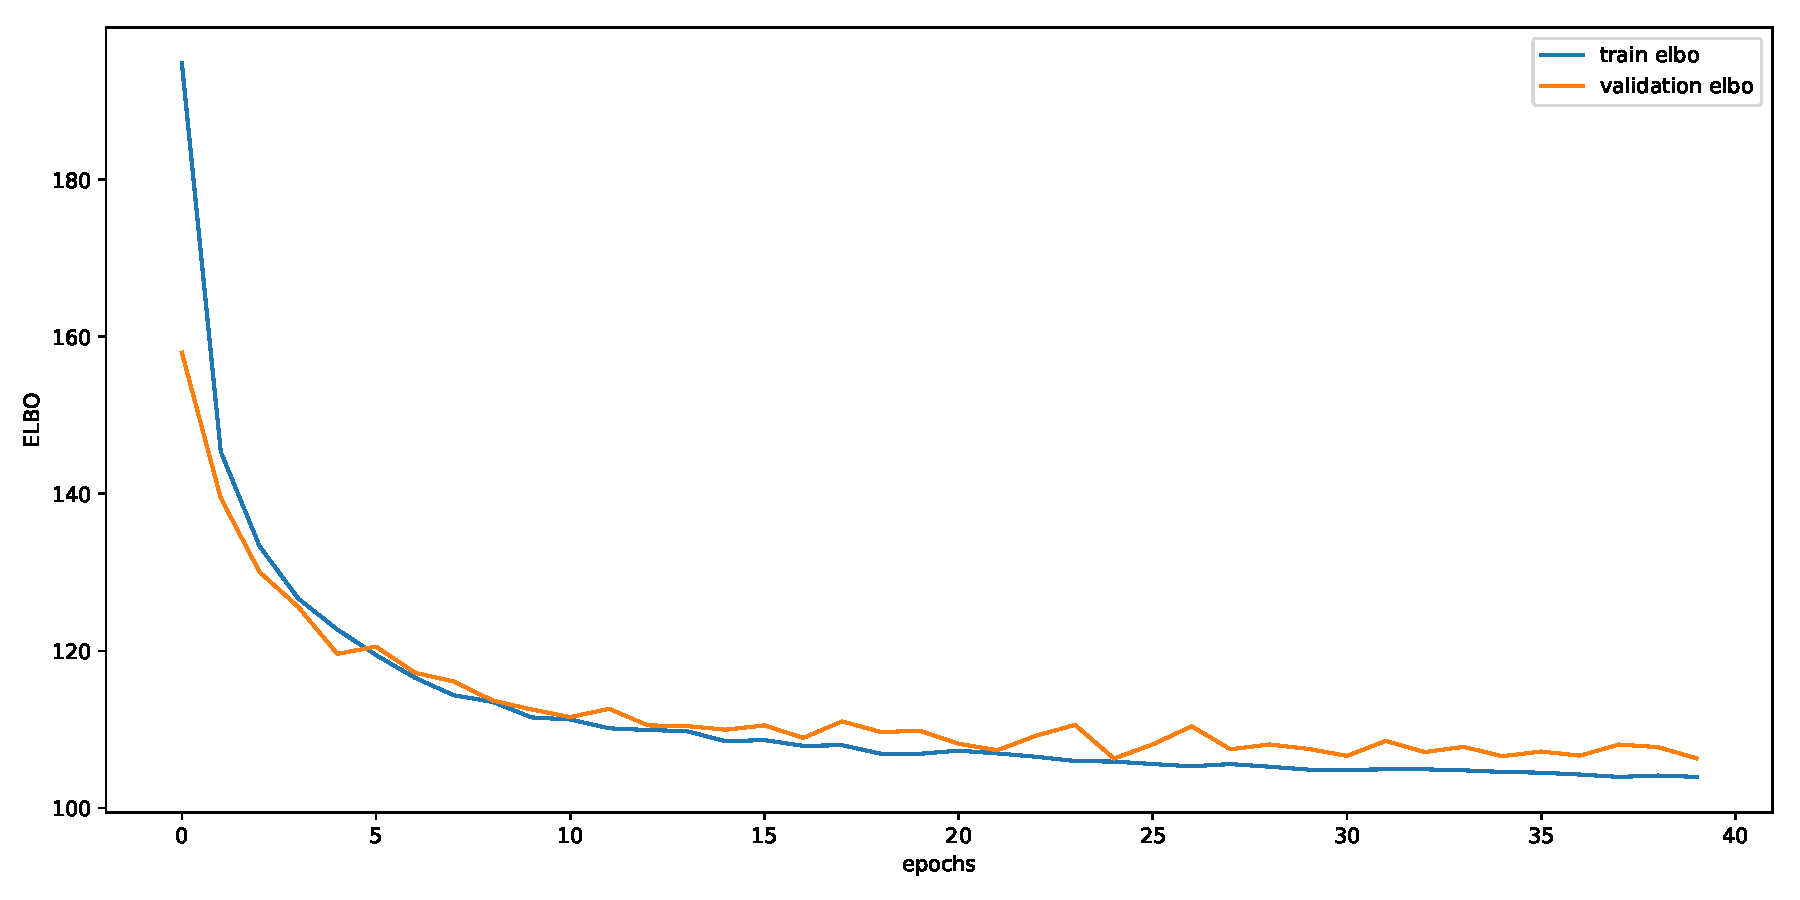
\includegraphics[scale=0.4]{img/elbo.pdf}
      \caption{Plot of the training and evaluation ELBO curves throughout the $40$ epochs of training.}
      \label{fig:elbo}
  \end{figure}

  \item
  Here I plot $25$ samples from the model at three equidistant moments during training: on the first epoch, on the $20^{\text{th}}$ epoch, and on the last epoch. The samples are shown in Figure \ref{fig:samples}.

  \begin{figure}
  \centering
  \begin{subfigure}
    \centering
    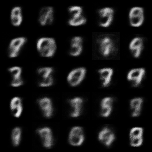
\includegraphics[width=.3\linewidth]{img/samples_epoch_00.png}
  \end{subfigure}
  \begin{subfigure}
    \centering
    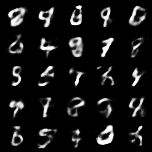
\includegraphics[width=.3\linewidth]{img/samples_epoch_19.png}
  \end{subfigure}
  \begin{subfigure}
    \centering
    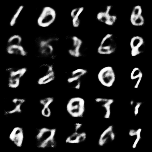
\includegraphics[width=.3\linewidth]{img/samples_epoch_39.png}
  \end{subfigure}
  \caption{$25$ samples from the VAE at different points during the training: from left to right at epoch $1$, $20$, and $40$.}
  \label{fig:samples}
  \end{figure}

  \item
  The 2-dimensional manifold for the VAE trained for $40$ epochs is shown in Figure \ref{fig:manifold}.

  \begin{figure}[ht]
      \centering
      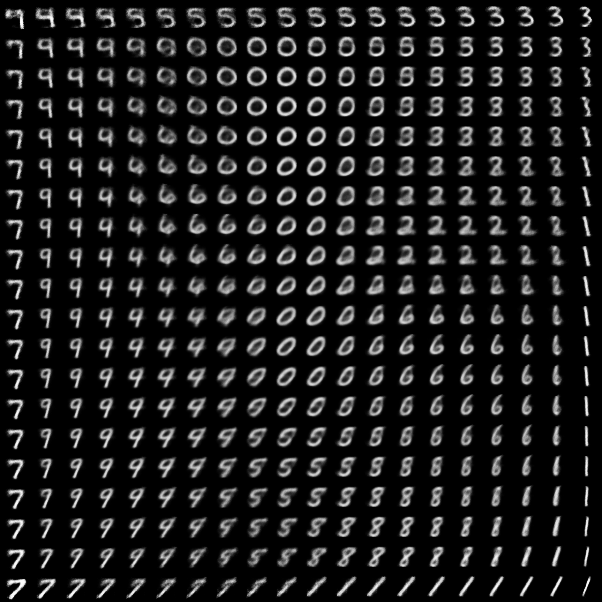
\includegraphics[scale=0.4]{img/manifold.png}
      \caption{Two-dimensional manifold for the VAE trained for $40$ epochs.}
      \label{fig:manifold}
  \end{figure}
\end{enumerate}


%################################# NEW SECTION ##################################
\section{Generative Adversarial Networks}

\begin{enumerate}[label=\textbf{2.\arabic*}]
  \item
  The generator takes as input a vector $\bm{z}$ sampled from some noise distribution. It outputs, in our case, an image of the same size and value range as the ones in the training set.

  The discriminator takes as input an image of the same type as the output of the generator (which may be the output of the generator or an actual image from the training set), and returns a score indicating how confident it is about the image being real or generated.
\end{enumerate}

%###################### NEW SUBSECTION #######################
\subsection{Training objective: A Minimax Game}

\begin{enumerate}[label=\textbf{2.\arabic*}]
  \setcounter{enumi}{1}
  \item
  The first term, $\mathbb{E}_{p_{data}(x)} \left[\log D(X) \right]$, refers to the expectation of the log-likelihood that the discriminator will successfully identify real pictures, given the distribution of the data.

  The second term, $\mathbb{E}_{p_{z}(z)} \left[\log (1 - D[G(Z)]) \right]$ refers to the expectation of the log-likelihood that the discriminator will successfully identify the generated images, given the noise distribution that they are being generated from.

  \item
  From the perspective of game theoretical perspective, in the ideal scenario after convergence the generator and discriminator should have reached the Nash equilibrium. Since this is a MiniMax game, we know that this occurs when the two parties win equally as likely, meaning that $D(X) = \frac{1}{2}$ and $D[G(Z)] = \frac{1}{2}$

  This conclusion would be reached if the two models were trained in such a way that they both reach peak performance, at which point both win equally as often.

  \item
  The problem with the second term arises from the fact that the discriminator is much easier to train compared to the generator. As such, it may happen that the second term saturates quickly, leaving a gradient of $0$ so that the generator can't learn anymore. At that point, the generator's performance plateaus.

  A solution is to use a different loss function for the generator. Namely, we can use $\log D(G[Z])$, which should be maximized instead of being minimized. Using this, the generator receives a strong gradient during backpropagation even if the discriminator has a perfect score (i.e. $\lim_{x\to 0} \del{\log x}{x} = \infty$)

\end{enumerate}

%###################### NEW SUBSECTION #######################
\subsection{Building a GAN}

\begin{enumerate}[label=\textbf{2.\arabic*}]
  \setcounter{enumi}{4}
  \item
  I did not have the time to implement the GAN.

  \item

  \item
\end{enumerate}


%################################# NEW SECTION ##################################
\section{Generative Normalizing Flows}

%###################### NEW SUBSECTION #######################
\subsection{Change of variables for Neural Networks}

\begin{enumerate}[label=\textbf{3.\arabic*}]
  \item
  For the multivariate case, the only two changes to apply are the use of vector notation, and the use of the absolute value of the determinant of the Jacobian instead of that of the derivatives themselves. As such, for eq. 16 we have:

  \begin{align*}
    \vec{\bm{z}} &= f(\vec{\bm{x}}) \\
    \vec{\bm{x}} &= f^{-1}(\vec{\bm{z}}) \\
    p(\vec{\bm{x}}) &= p(\vec{\bm{z}}) \abs{\det \del{\vec{\bm{f}}}{\vec{\bm{x}}}}
  \end{align*}

  While for eq. 17 we have:

  \begin{align*}
    \log p(\vec{\bm{x}}) &= \log p(\vec{\bm{z}}) + \sum_{l=1}^L \log \abs{\det \del{\vec{\bm{h}}_{l}}{\vec{\bm{h}}_{l-1}}}
  \end{align*}

  \item
  The first criterion is that $f(\vec{\bm{x}})$ needs to be invertible. The second is that the Jacobian matrix should be square, otherwise we can't compute its determinant. This second constraint implies that the dimensionality of $\vec{\bm{x}}$ and $\vec{\bm{z}}$ should be the same. Furthermore, the determinant of the jacobian should be non-zero, since that would make the last logarithm undefined.

  \item
  The problem with optimizing the aforementioned equation is that both computing the Jacobian and computing the determinant are very computationally expensive. Computing the Jacobian is in $\mathcal{O}(n^3)$. Computing the determinant is also expensive but its computational complexity varies depending on the Jacobian's properties.

  \item
  The consequence of this would be an uneven distribution mapping. In other words, since the pixel values are discrete, we don't have a complete distribution. When mapping the initial (quantized) distribution through the various normalizing flows, this will produce uneven and sparse intermediate and final distributions, so that it will be very hard to sample from them.

  In order to fix this problem, the paper cited in the question proposes among others a technique called \textit{uniform quantization}. For an input image where each of the $D$ pixels take an integer value in the range $(0, 255)$, this means adding $\epsilon \sim \mathcal{U}[0, 1)^D$ to the input. The effect is to fill the spaces inbetween discrete pixel values, this producing a smoother distribution.
\end{enumerate}

%###################### NEW SUBSECTION #######################
\subsection{Building a flow-based model}

\begin{enumerate}[label=\textbf{3.\arabic*}]
  \setcounter{enumi}{4}
  \item
  During training the flow-based model takes as input a data point from the dataset (e.g. an image). The output, after the sample has been mapped through the model's flows, should be a data point of the same dimensionality but belonging to a different distribution, one that allows for easier sampling.

  During inference time the process is reversed: we feed the model a data point sampled from a noise distribution of the same dimensionality as the training examples, and we obtain as output an image of that same dimensionality that resembles the ones from our training dataset. Note that during inference the flow is reversed compared to the training configuration.

  \item
  During training we want to iteratively perform these steps:

  \begin{enumerate}[label=\arabic*.]
    \item Feed samples from our dataset into the flow-based model, and receive a data point from the output distribution.

    \item Since we computed the determinants of the Jacobian for each pair of consecutive flows during forward propagation, we use those instead of computing them again. We plug them into our loss function (i.e. the negative log-likelihood) along with the log-probability of the output data point. We can now backpropagate the loss through our model.
  \end{enumerate}

  During inference we will do the opposite:

  \begin{enumerate}[label=\arabic*.]
    \item Feed a data point sampled from the prior distribution into the reverse of the flow.

    \item As output we obtain a data point similar to the data points in our original dataset.
  \end{enumerate}

  \item
  I did not have the time to implement the GNF.

  \item
\end{enumerate}


%################################# NEW SECTION ##################################
\section{Conclusion}

\begin{enumerate}[label=\textbf{4.\arabic*}]
  \item
  In this assignment we explored three generative models, which approach the task of approximating the log-likelihood of the data in different ways.

  Variational Auto Encoders do this by optimizing a quantity that can be brought back to the log-likelihood of the data: the ELBO. By modelling a latent variable to encode the data, we can maximize the ELBO and train a generator for new datapoints. Hence, the log-likelihood of the data is modelled indirectly by manipulating distributions and their divergences.

  Generative Adversarial Networks, on the other hand, don't model the log-likelihood of the data at all. This configuration involves a generative network and a discriminative network. The two compete in a zero-sum MiniMax game, in which the generator learns to mimic the real data as closely as possible by making the discriminator classify its output as real data.

  Generative Normalizing Flows are the only one of the three models that directly maximizes the log-likelihood of the data. By mapping the original data's complex distribution through a series of invertible functions, this model simplifies the distribution (effectively mapping it to noise). By doing this, it makes it possible to sample from the noise distribution and feed the sampled data point through the reverse model, in order to generate novel samples.
\end{enumerate}

\end{document}
